\section{Constraints on Fold
Features}\label{constraints-on-fold-features}

Constraints are central to the implementation of Foldlings' algorithms,
which help our software provide an accurate preview of sketches, and
ensure that designs created with Foldlings will fold correctly. As an
educational tool, one of the primary benefits of our software might be
the development of an intuitive understanding of the limits of paper.

\subsection{Geometric Constraints}\label{geometric-constraints}

Several geometric constraints drive Foldling's algorithms. These
constraints are the core reason for the difficulty of creating designs
manually; a key advantage of our system is that these constraints are
resolved automatically.

\subsubsection{Box Fold}\label{box-fold}

\begin{figure}[htbp]
\centering
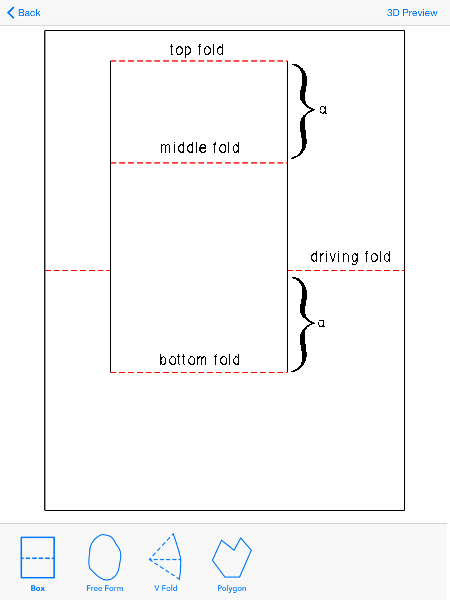
\includegraphics{figures/45_Tech_Constraints/boxfoldConstraints.pdf}
\caption{Geometric constraints for freeform features}
\end{figure}

A box fold is constrained by a relationship between its folds. Given a
top fold and bottom fold at fixed height, with a driving fold with a
height between the other two folds, the vertical distance between the
bottom fold and the driving fold must be equal to the distance between
the top fold and the middle fold of the feature.

This 90-degree angle constraint applies equally to freeform and polygon
features (at least, those that span a fold).

\subsubsection{Freeform}\label{freeform}

\begin{figure}[htbp]
\centering
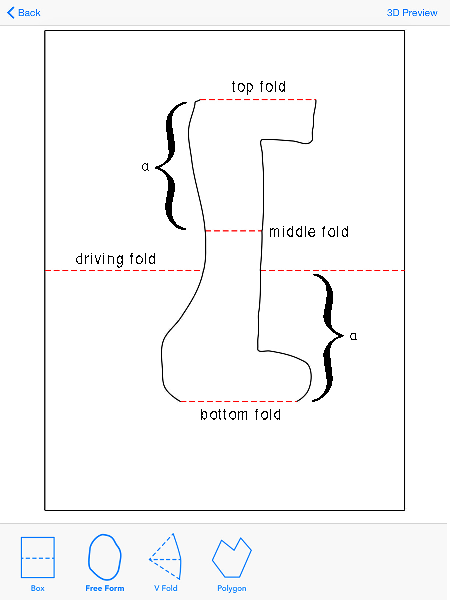
\includegraphics{figures/45_Tech_Constraints/freeformConstraints.pdf}
\caption{Geometric constraints for freeform features}
\end{figure}

Freeform fold heights are calculated similarly to those in a box fold.
After performing truncation \footnote{described
  \textbf{\textgreater{}\textgreater{}TODO: CITE}} to place the top and
bottom folds of the freeform shape, we apply the ninety-degree
constraint to place the middle fold in the feature. Of course, holes are
not bound by this constraint, because they do not have a driving fold.

As with all features, validity constraints are separate from geometric
constraints. Freeform shapes that intersect themselves do not have a
place for the middle fold, but by performing validity checks before
solving for geometric constraints, we avoid many problems and edge cases
that would otherwise occur.

\subsubsection{Polygon}\label{polygon}

\begin{figure}[htbp]
\centering
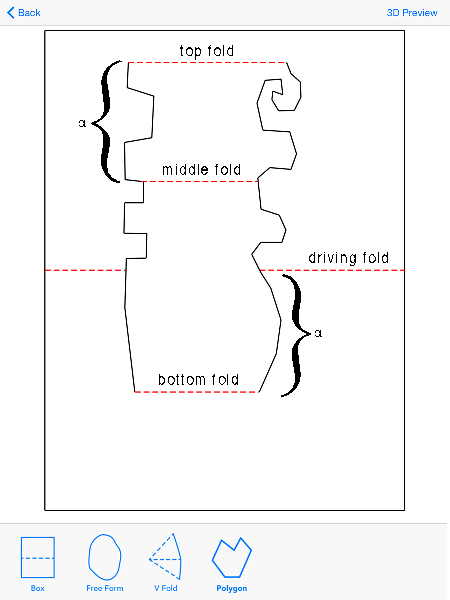
\includegraphics{figures/45_Tech_Constraints/polygonConstraints.pdf}
\caption{Geometric constraints for polygon features}
\end{figure}

The same constraints that apply to freeform shape apply to polygons.
Although the edges are constructed differently, polygons are essentially
a subset of freeform shapes, composed only of straight lines.

\subsubsection{V-Fold}\label{v-fold}

\begin{figure}[htbp]
\centering
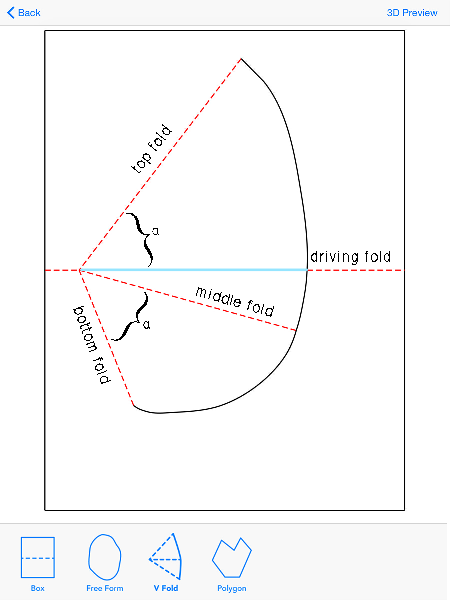
\includegraphics{figures/45_Tech_Constraints/vfoldConstraints.pdf}
\caption{Geometric constraints for freeform features}
\end{figure}

Although a v-fold also folds from zero to 180 degrees with the card, its
planes moves at non-orthogonal angles. The constraint of folds in a
v-fold feature is therefore based on angle rather than height.

The simplest case of v-folds --- and the one most popularly constructed
by our user testers using manual methods --- is a symmetric v-fold. In
this case, the top and bottom angles of the fold are equal. The shape
approximates an isosceles triangle.

In the more complex case, the angles between the two diagonal folds and
the driving fold differ. Andrew Glassner demonstrates that for any
``single slit mechanism,'' the angle from the driving fold to either the
top or bottom fold must be equal to the angle between the opposite fold
and the middle fold (\citet{glassner1998interactive}, 3). This
constraint is only solvable if the sum of the angles between each
diagonal fold and driving fold is less than 180º. Intuitively, this
constraint is not dissimilar from the constraint for box folds ---
position of the middle fold is constrained by the driving fold's
relationship to the top and bottom folds.

\subsection{Physical Constraints}\label{physical-constraints}

In addition, the physicality of paper place constraints on where cuts
and folds can be placed. Depending on the manufacture method, there is
some minimum line length that can be cut or folded, and some minimum
distance folds and cuts must be apart. These depends on a wide number of
variables ranging from paper thickness to manufacture method (for
example, laser cutters have a higher tolerance for closely-drawn lines).
Even within a specific technology, there is also a wide variation in
cutting precision.

\begin{figure}[htbp]
\centering
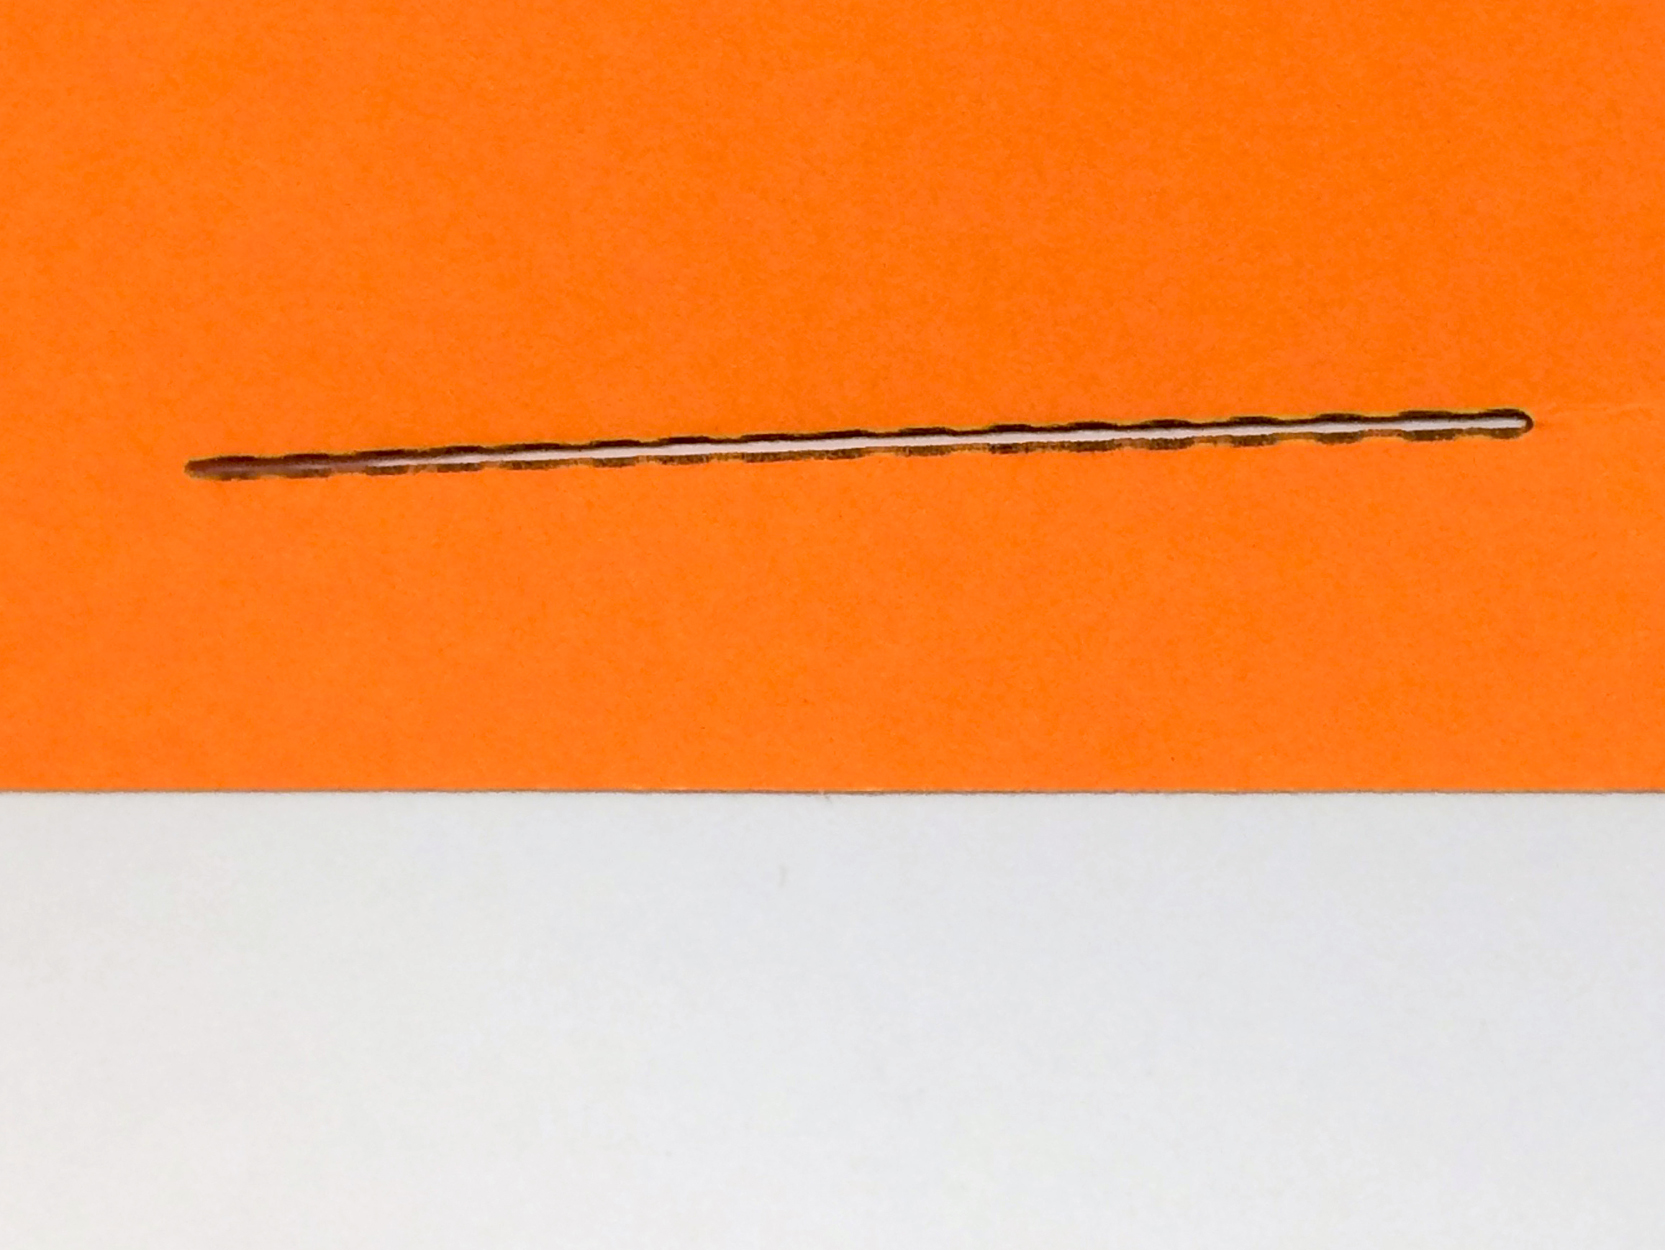
\includegraphics{figures/45_Tech_Constraints/tooclosecuts.jpg}
\caption{A malformed laser-cut fold. This is supposed to be a dotted
line, but because the dots were too close together, the dot have merged
to become a single cut.}
\end{figure}

In our software, we take this into account through the minimum edge
length. This. Due to the wide In addition, we . We currently

Physical. Obvious . Minimum edge length. This depends on the laser
cutter

\textbf{\textgreater{}\textgreater{}TODO: Figure showing problem}
